\documentclass[14pt]{extarticle}
\usepackage{graphicx}
\usepackage{setspace} %para pequenos espaçamentos
\usepackage[document]{ragged2e} %para alinhamentos
\usepackage[margin=1.5cm]{geometry} % margem em todos os lados do documento
\usepackage{indentfirst} %para indentar o primeiro paragrafo numa section
\usepackage{listings} %code


\title{Programação\\
        Relatório - Jogo do Semáforo}
\date{}
\renewcommand*\contentsname{} %para tirar a palavra "Contents"


\begin{document}
\setlength{\parindent}{1em} % indentação global dos paragrafos
\setlength{\parskip}{0.5em} %espaço entre paragrafos, margem em cima dos paragrafos

%Página Principal
\maketitle

\begin{figure}[h]
    \centering
    
\includegraphics[width=0.50\textwidth]{logo}
\end{figure}

\vspace{50mm}

\begin{center}
  Docente: Francisco Pereira\\
  Trabalho realizado por: Nelson Simão nº2020132648- LEI\\
\end{center}

\newpage
\begin{center}
  \Large Indíce
\end{center}


\tableofcontents

\newpage
\section{Principais estruturas de dados}
No programa existem 5 estruturas de dados principais: struct plays, struct player, struct coordinates, struct list\_head e struct list\_node.
\subsection{struct plays}
\begin{figure}[h]
    \centering
    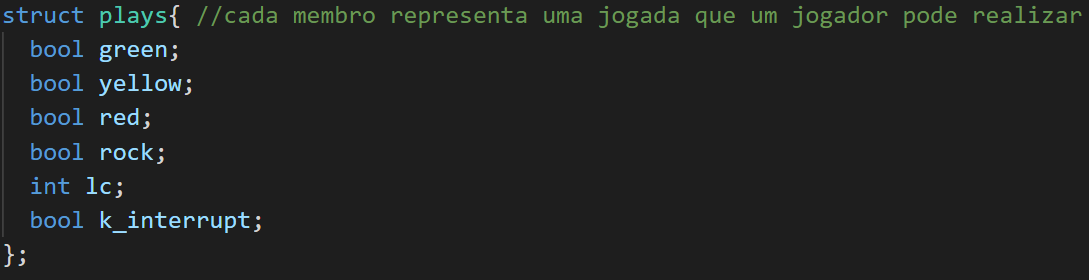
\includegraphics[width=\textwidth]{plays}
\end{figure}
Esta estrutura serve para indicar que jogadas um jogador pode realizar ao longo do jogo.
\begin{itemize}
\item \textbf{bool green} - toma o valor 1 se o jogador puder colocar uma peça verde no tabuleiro, 0 se nao o puder fazer
\item \textbf{bool yellow} - toma o valor 1 se o jogador puder trocar uma peça verde por uma amarela no tabuleiro, 0 se nao o puder fazer
\item \textbf{bool red} - toma o valor 1 se o jogador puder trocar uma peça verde por uma amarela no tabuleiro, 0 se nao o puder fazer
\item \textbf{bool rock} - toma o valor 1 se o jogador puder colocar uma pedra no tabuleiro, 0 se nao o puder fazer, um jogador só pode realizar esta jogada uma vez por jogo
\item \textbf{int lc} - numero de colunas ou linhas que o jogador pode inserir no tabuleiro, um jogador só pode realizar esta jogada 2 vezes por jogo
\item \textbf{bool k\_interrupt} - toma o valor 1 se o jogador puder ver as k jogadas anteriores ou se puder interromper o jogo, ambas jogadas só podem ser feitas após o 1º turno
\end{itemize}

\newpage
\subsection{struct player}
\begin{figure}[h]
    \centering
    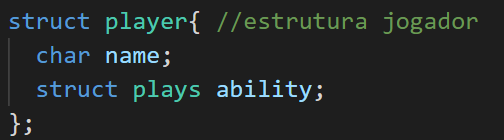
\includegraphics[width=0.75\textwidth]{player}
\end{figure}
Estrutura que representa um jogador. Contem outra estrutura(\textbf{struct plays}) que representa as jogadas que o jogador pode realizar, como já foi mencionado anteriormente. \textbf{char name} representa o nome do jogador, 'A' ou 'B'.
\subsection{struct coordinates}
\begin{figure}[h]
    \centering
    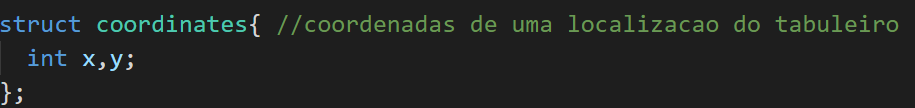
\includegraphics[width=0.75\textwidth]{coordinates}
\end{figure}
Esta estrutura serve para guardar as coordenadas de uma celula do tabuleiro, (x,y).
\newpage
\subsection{struct list\_node}
\begin{figure}[h]
    \centering
    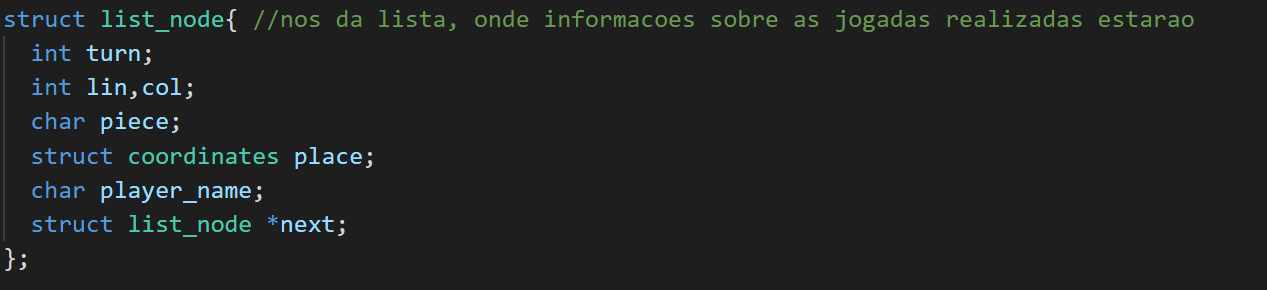
\includegraphics[width=\textwidth]{node}
\end{figure}
Para implementar a funcionalidade de "visualizar o estado do tabuleiro nas K jogadas anteirores" e ainda a "exportação para um ficheiro de texto", era obrigatório a implementação de uma lista ligada. A estrutura \textbf{struct list\_node} representa um nó desta lista ligada. O objetivo desta lista ligada é armazenar informação sobre as jogadas realizadas ao longo do jogo.
\begin{itemize}
\item \textbf{int turn} - Turno atual, representa tambem o indice do nó na lista
\item \textbf{int lin} - Número de linhas do tabuleiro no turno atual
\item \textbf{int col} - Número de linhas do tabuleiro no turno atual
\item \textbf{char piece} - Carater que representa a peça/jogada realizada nesse turno(se for esse o caso, ex: se \textbf{piece}=='C' foi adicionada uma coluna e nenhum carater foi colocado no tabuleiro)
\item \textbf{struct coordinates place} - Coordenadas do tabuleiro em que a peça foi colocada
\item \textbf{struct list\_node *next} - Ponteiro para o próximo nó
\end{itemize}

\newpage
\subsection{struct list\_head}
\begin{figure}[h]
    \centering
    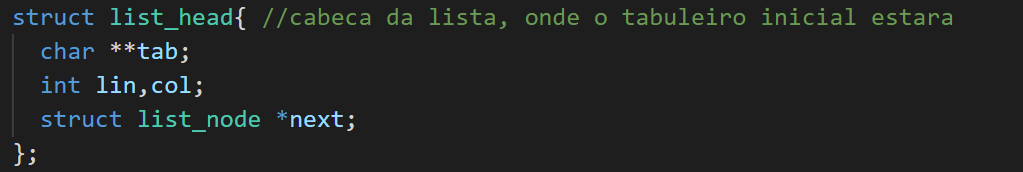
\includegraphics[width=\textwidth]{head}
\end{figure}
A estrutura \textbf{struct list\_head} representa a cabeça da lista ligada. A lista ligada implementada neste programa é uma "lista ligada mista", ou seja, a cabeça da lista é diferente dos seus nós. A lista ligada será explicada na secção 2.
\begin{itemize}
\item \textbf{char **tab} - Este ponteiro para ponteiro aponta para um array bidimensional alocado dinamicamente, e representa o tabuleiro do jogo no inicio do jogo.
\item \textbf{int lin} - Número de linhas de \textbf{tab}
\item \textbf{int col} - Número de colunas de \textbf{tab}
\item \textbf{struct list\_node *next} - ponteiro para um nó da lista
\end{itemize}

\newpage
\section{Estruturas dinâmicas implementadas}
Este programa contém duas estruturas dinâmicas: o array bidimensional que representa o tabuleiro de jogo e a lista ligada que armazena informação sobre as jogadas realizadas ao longo do jogo.
\subsection{char **tab}
Esta estrutura dinâmica, um vetor bidimensional alocado dinamicamente, representa o tabuleiro do jogo e, sendo que é alocado dinamicamente, é possivel a adição de linhas e colunas. Segue-se um esquema do tabuleiro com 3 linhas e 3 colunas:
\begin{figure}[h]
    \centering
    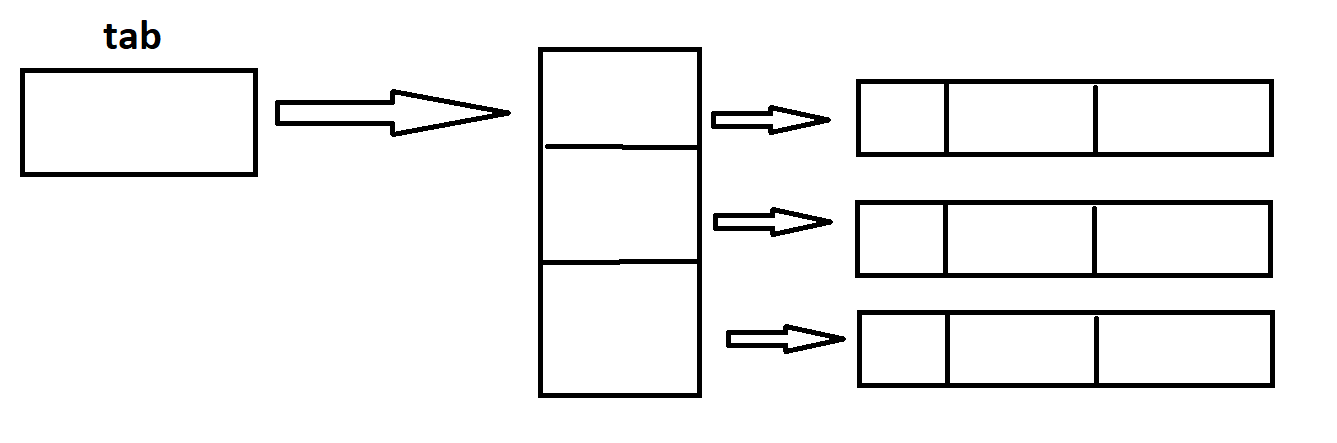
\includegraphics[width=\textwidth]{tab}
\end{figure}

É possível observar então que \textbf{tab} aponta para um array alocado dinamicamente de \textbf{char *} e cada um dos elementos deste array aponta para outro array alocado dinamicamente de \textbf{char}. Através de simples aritmética de ponteiros podemos perceber que podemos aceder ao elemento da linha \textbf{i}, coluna \textbf{j}, com \textbf{tab[i][j]}. 
Escusado dizer que um acesso tao simples a um elemento permite uma grande simplificacão das operações no tabuleiro. Este fator, aliado à simplicidade da estrutura de dados(que no fundo nao difere muito de um array bidimensional alocado na stack) foi o motivo pelo qual optei por esta estrutura de dados para representar o tabuleiro de jogo. 

\newpage
\subsection{lista ligada}
A lista ligada serve para um jogador, puder visualizar o estado do tabuleiro nas \textbf{K} jogadas anteriores e ainda para poder exportar a sucessão de estados do tabuleiro para um ficheiro .txt. 

A lista ligada por mim escolhida é uma lista ligada "mista", ou seja, a cabeça da lista é diferente dos nós que a compõem. A cabeça da lista irá armazenar o tabuleiro vazio, tal e qual como ele estava no principio do jogo(quadrado e com um numero aleatório de linhas) e irá armazenar também as suas dimensões (linhas e colunas). Cada nó da lista, que é de um tipo diferente da cabeça, corresponde a um turno, e cada nó, armazena informação sobre a jogada realizada nesse turno(ver definição de um nó na secção anterior). O objetivo desta separação é muito simples.

Segue-se agora um exemplo que mostra a utilidade da lista, não pretendo explicar todas as funções subjacentes às operações que irei mostrar, pretendo é exemplificar um exemplo de aplicação da lista ligada.

Suponhamos então que estamos no turno 3, vez do jogador A, e o tabuleiro encontra-se no seguinte estado:
\begin{figure}[h]
    \centering
    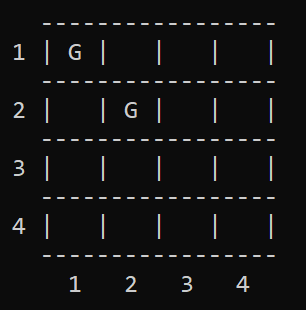
\includegraphics[width=0.25\textwidth]{tab1}
\end{figure}

A lista encontra-se neste estado:
\begin{figure}[h]
    \centering
    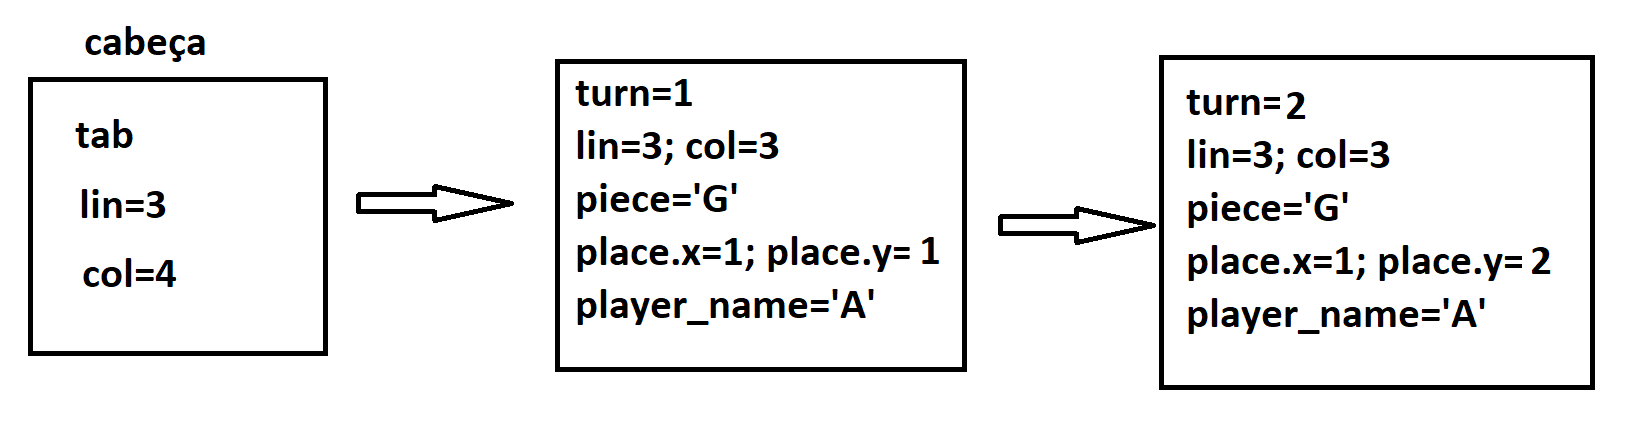
\includegraphics[width=\textwidth]{list1}
\end{figure}

Na cabeça \textbf{tab} está a apontar para um tabuleiro alocado dinamicamente de dimensao 4x4.

Quando o jogador A seleciona a opção de ver as 2 jogadas anteriores, é chamada uma função que conforme a informação em cada nó, vai alterando o tabuleiro que está na cabeça da lista até chegar ao nó com \textbf{turn}=2, e enquanto atualiza o tabuleiro que esta na cabeça da lista, vai escrevendo esse tabuleiro e informação sobre a jogada realizada nesse turno na consola. Para este exemplo obtemos então:

\begin{figure}[h]
    \centering
    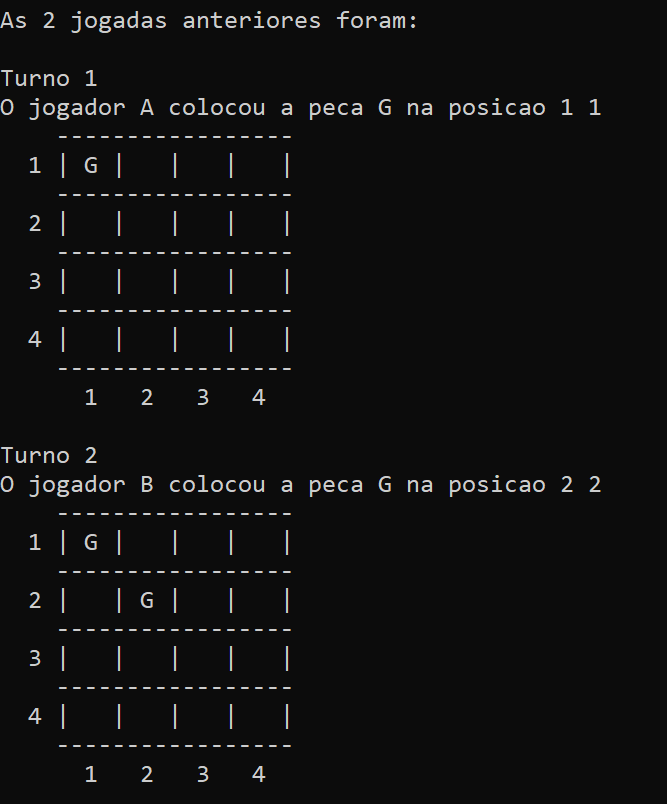
\includegraphics[width=0.50\textwidth]{list2}
\end{figure}

No final de toda esta operação, o tabuleiro presente na cabeça volta ao estado em que estava no inicio do jogo. Com uma lista assim fui capaz de mostrar informação completa e detalhada sobre a sucessão de estados do tabuleiro na consola, e também, no ficheiro de texto(o procedimento é semelhante mas mais linear). O facto de poder escrever informação detalhada sobre as jogadas realizadas, foi o meu motivo de escolha desta lista ligada.

\newpage
\section{Funcionamento do Programa}
No inicio do programa, a função \textbf{main} apresenta um menu ao utilizador que lhe permite escolher se, quer jogar contra outro jogador, se quer jogar contra o computador, se quer ver as regras do jogo ou se quer sair do programa. Nesta secção irei-me focar nas opções de jogo já que as duas outras são muito simples. A função \textbf{main} apenas tem o propósito de receber input do utilizador, validá-lo, e conforme a opção escolhida, supondo que o utilizador quer jogar, chamar a função \textbf{game(bool game\_mode, bool resume}.

O jogo decorre na função \textbf{game} onde:
\begin{itemize}
\item \textbf{bool game\_mode} - 0 indica que o jogo deverá se realizar a dois jogadores humanos, 1 indica que o jogo será contra o computador
\item \textbf{bool resume} - 0 indica que é para começar um jogo novo, 1 indica que é para continuar um jogo anterior
\end{itemize}

Se o utilizador não quiser continuar o jogo anteriror e escolher a opção de jogar contra o computador, a função \textbf{main} chamará a função \textbf{game} com \textbf{game\_mode=1, resume=0}.

Se o ficheiro \textbf{jogo.bin} existir, quer dizer que há um jogo por retomar, e nesse caso a função main apenas pergunta ao utilizador ser quer continuar o jogo. Se o utilizador nao quiser então o menu normal ser-lhe-à apresentado, caso contrário \textbf{main} acede a \textbf{jogo.bin}, determina o modo de jogo e invoca a função \textbf{game} com os argumentos apropriados.

Quando o controlo passa para \textbf{game}, esta função dependendo dos parametros com que foi chamada inicia ou retoma um jogo. Por exemplo: se a função game foi chamada com \textbf{game\_mode=0, resume=1}, então a função chama outras funções auxiliares que inicializão as variaveis necessárias ao funcionamento do jogo com os valores que elas tinham quando o jogo foi interrompido e, se essa operação for um sucesso, o jogo continua normalmente. Se o jogo for contra o computador, por exemplo, em vez de \textbf{game} pedir uma jogada ao jogador 'B', pede uma jogada ao "jogador autmático".

O jogo então sucede normalmente, a pedir jogadas a ambos os jogadores alternadamente, e o tabuleiro de jogo vai sendo alterado. No final de um turno é adicionado um nó à lista ligada, com informação sobre as jogadas realizadas nesse turno. O jogo acaba quando um dos jogadores vencer, vence o jogador que conseguir formar uma linha, coluna ou diagonal com peças da mesma cor. Quando isso acontece é pedido ao utilizador um nome para um ficheiro .txt onde informação sobre o jogo ficará armazenada. Após isto o programa termina.

\newpage

\section{Pequeno Manual de Utilização}
Assim que o programa começa é apresentado o seguinte menu ao utilizador:
\begin{figure}[h]
    \centering
    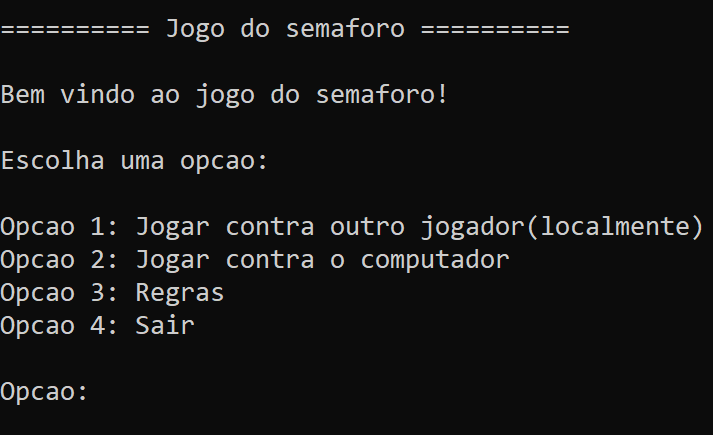
\includegraphics[width=0.50\textwidth]{menu}
\end{figure}

Se o utilizador escolher a opção 3, as regras do jogo são apresentadas na consola e ainda é dada a possibilidade de as regras serem guardadas num ficheiro .txt para poderem ser consultadas a meio do jogo. No final de as regras estarem mostradas o menu volta a aparecer.

Independentemente da opção de jogo escolhida pelo utilizador, opção 1 ou opção 2, o resultado será sempre o mesmo:
\begin{figure}[h]
    \centering
    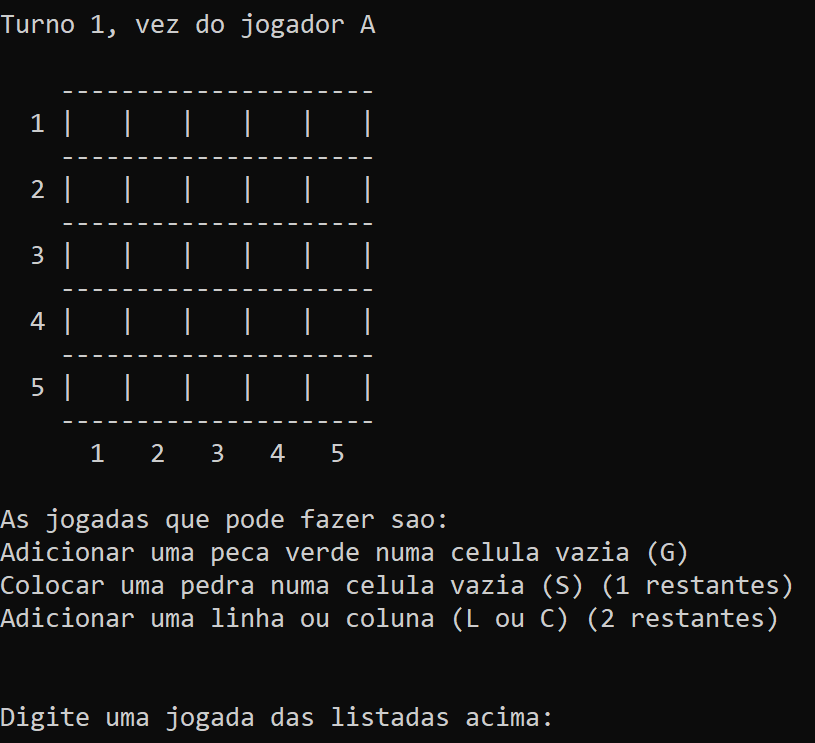
\includegraphics[width=0.50\textwidth]{game1}
\end{figure}

O jogador A é sempre um jogador humano e é o primeiro a começar. É apresentado um desenho do tabuleiro, incialmente vazio, e as jogadas que o jogador atual pode fazer são apresentadas no ecrã, com uma descrição sobre a jogada e o carater entre "()" associado a essa jogada.

Para jogar basta então pressionar um carater válido:
\begin{figure}[h]
    \centering
    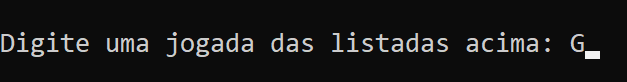
\includegraphics[width=0.50\textwidth]{game2}
\end{figure}

Se for o caso, como neste exemplo, inserir as coordenadas em que a peça deve ser colocada no tabuleiro:
\begin{figure}[h]
    \centering
    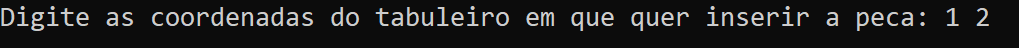
\includegraphics[width=0.50\textwidth]{game3}
\end{figure}

E após isso o tabuleiro será atualizado, o turno incrementado, e passamos para a vez do jogador B.
\begin{figure}[h]
    \centering
    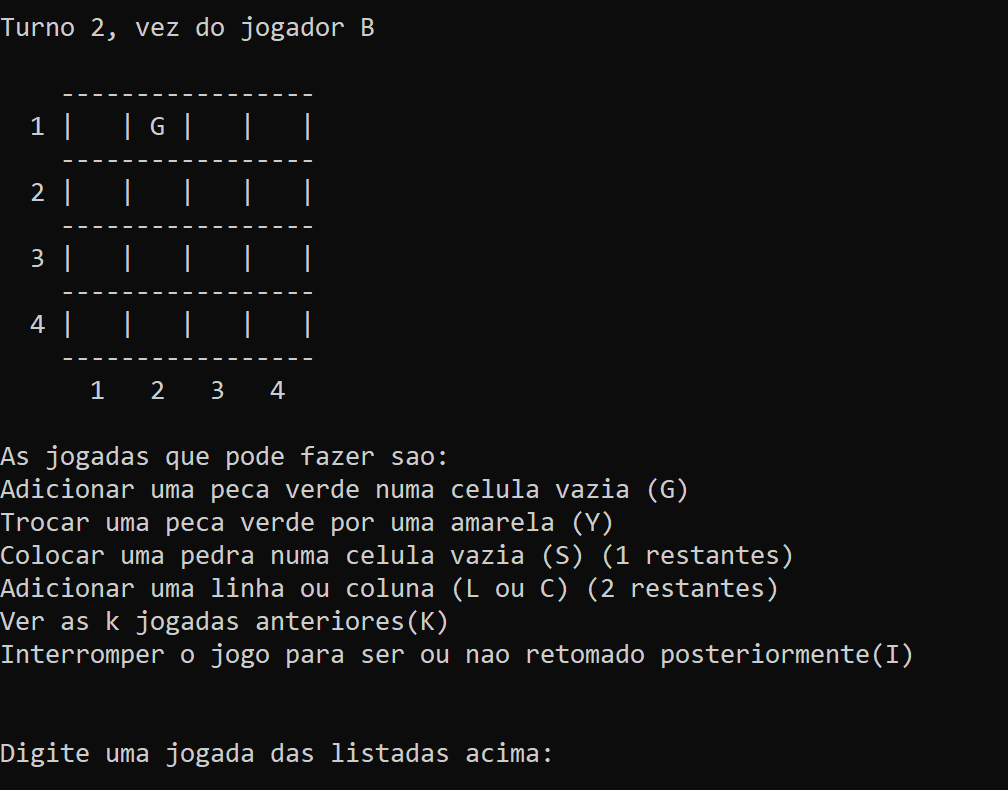
\includegraphics[width=0.60\textwidth]{game4}
\end{figure}

Podemos ver que o jogador B já pode realizar jogadas que o jogador A nao pôde realizar. Isto deve-se a uma peça verde ter sido inserida no tabuleiro o que implica que o jogador B poderá então trocar essa peça por uma amarela. Também podemos verifcar que o jogador B já pode interromper o jogo e ver as K jogadas anteriores, isto deve-se ao facto de estarmos no turno 2. Não faria muito sentido interromper o jogo no primeiro turno nem era possivel visualizar qualquer jogada anterior no primeiro turno.
\newpage
Qualquer tentativa de inserir um carater invalido, um carater que representa uma jogada que o jogador nao pode realizar no momento ou umas coordenadas inválidas, serão bloqueadas e uma mensagem de erro será exibida a pedir ao utilizador que insira esses dados corretamente.
\begin{figure}[h]
    \centering
    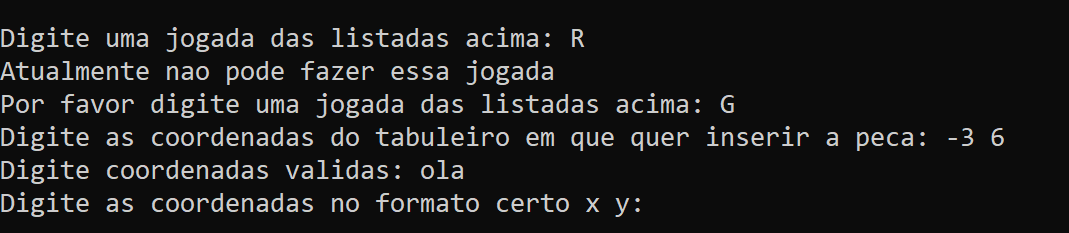
\includegraphics[width=0.60\textwidth]{game5}
\end{figure}

Se escolher o carater 'I', será exibida uma mensagem a indicar se foi possível guardar informação para retomar o jogo num ficheiro binário, ou uma mensagem de erro se tal operação nao foi possível, em ambos os casos o programa terminará.

No final do jogo, vitória de um jogador, é apresentado o tabuleiro atualizado e uma mensagem a indicar que jogador venceu:
\begin{figure}[h]
    \centering
    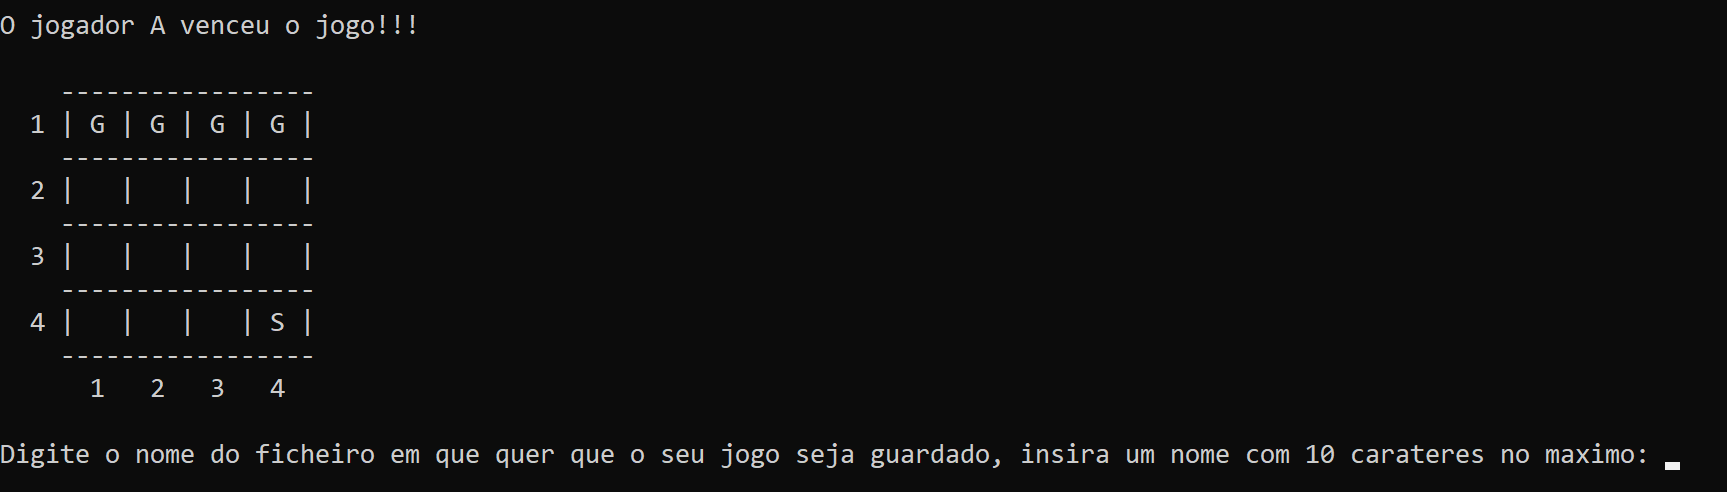
\includegraphics[width=0.75\textwidth]{game6}
\end{figure}

E é pedido ao utilizador o nome para um ficheiro que irá guardar a sucessão de estados do tabuleiro. São lidos no máximo 10 carateres e a extensão .txt é adicionada pelo programa.

\newpage
Segue-se uma imagem do ficheiro .txt:
\begin{figure}[h]
    \centering
    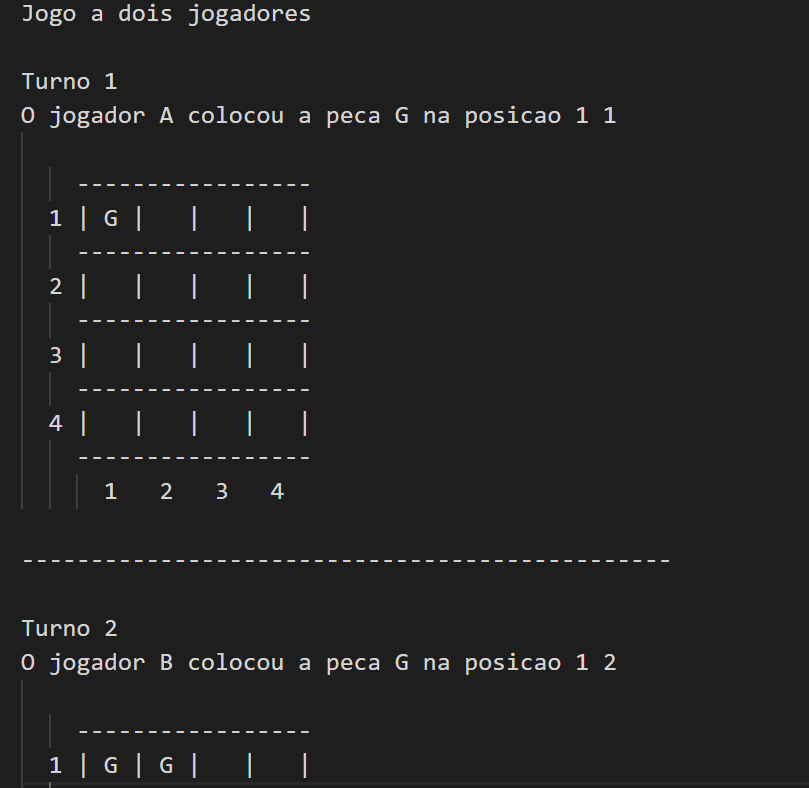
\includegraphics[width=0.50\textwidth]{game7}
\end{figure}

O jogo contra o computador não será ilustrado nesta secção. A única diferença deste modo de jogo é que o jogador A é o utilizador, e este joga contra o computador. Vale a pena salientar que o jogador automático realiza uma jogada válida aleatoriamente e que nunca irá interromper o jogo ou visualizar as K jogadas anteriores. De resto comporta-se como um jogador humano normal.


\end{document}